% Appendix: point-process background, as included in paper_v2.tex.
% Edited from appendix_point_process.tex (older draft): notation aligned with the
% paper (tau = Fano bin width, T = service time), numbers replaced by the paper's own,
% and the older draft's data, model-class and diagnostic-panel sections left out.

\section{Point-process background}
\label{app:pp-background}

This appendix defines the terms the paper uses for arrival streams: the Poisson,
renewal and Hawkes processes, the conditional intensity, the branching ratio, the Fano
factor and the Hurst exponent, and what it means to fit a Hawkes process. It assumes no
prior knowledge of point processes. Readers who know what a conditional intensity is can
go straight to Section~\ref{app:pp-canon}. Two notational points: $\tau$ is a bin width
for counting arrivals, and $T$ is reserved, as in the rest of the paper, for the service
time of a receiver.

\subsection{The Poisson process}
\label{app:pp-warmup}

\paragraph{The setup.} Watch packets arrive from a market-data feed and write down the
time of each arrival:
\begin{verbatim}
09:30:00.213    <- 1st arrival
09:30:00.451    <- 2nd
09:30:00.802    <- 3rd
09:30:01.014    <- 4th
09:30:01.317    <- 5th
...
\end{verbatim}
That list of timestamps is the object being modelled. Nothing else --- no prices, no
sides, only when.

\paragraph{The Poisson idea.} Suppose that in every very small slice of time there is a
small, \emph{independent} chance of an arrival. Independent means that whether an arrival
happens now does not depend on when the previous one came, on how many came in the last
minute, or on anything else about the past. The \emph{rate} of the process is a single
number, written $\mu$, in arrivals per second. At a rate of $300$ per second, on average
$300$ arrivals occur in each second. Three consequences follow from the independence.

\paragraph{(1) The gap between consecutive arrivals is exponentially distributed with
mean $1/\mu$.} At $\mu = 300$ per second the mean gap is
$$\text{mean gap} = \frac{1}{\mu} = \frac{1}{300/\mathrm{s}} \approx 3.3\ \mathrm{ms}.$$
The gap distribution is memoryless: however long one has been waiting, the expected time
to the next arrival is still $3.3$\,ms. The probability that a gap exceeds $\Delta$ is
$$\Pr(\text{gap} > \Delta) = e^{-\mu\,\Delta},$$
so at this rate $\Pr(\text{gap} > 3.3\,\mathrm{ms}) \approx 36.8\%$,
$\Pr(\text{gap} > 6.6\,\mathrm{ms}) \approx 13.5\%$ and
$\Pr(\text{gap} > 10\,\mathrm{ms}) \approx 5.0\%$. The probability that a gap is shorter
than a tenth of the mean is
$$\Pr\!\big(\text{gap} < \tfrac{1}{10}\,\text{mean}\big) = 1 - e^{-0.1} \approx 9.52\%,$$
whatever the rate. This is the Poisson benchmark used in Section~\ref{sec:setup-hawkes}
for how often two arrivals come nearly back to back; on the corpus the share is $73\%$.

\begin{figure}[H]
    \centering
    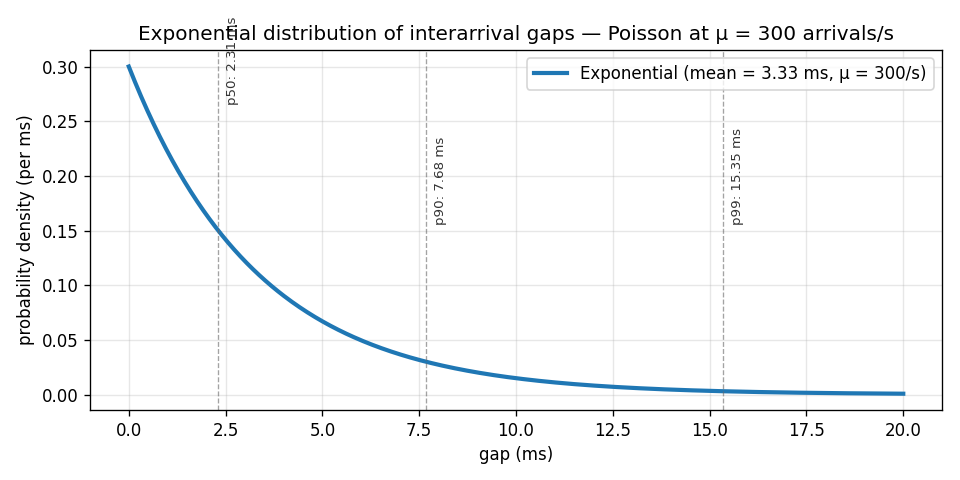
\includegraphics[width=0.75\textwidth]{figs/exponential_gaps.png}
    \caption{The exponential density of interarrival gaps for a Poisson process at $300$
    arrivals per second. Dashed vertical lines mark the median, $p_{90}$ and $p_{99}$.
    Half the gaps are shorter than the median of $2.3$\,ms and $10\%$ are longer than
    $7.7$\,ms. The CME packet stream has a different shape: far more mass near zero and a
    much heavier right tail (Figure~\ref{fig:tx-gaps}).}
    \label{fig:exponential-gaps}
\end{figure}

\paragraph{(2) The count in any bin of width $\tau$ is Poisson-distributed.} Let $C$ be
the number of arrivals in a bin of width $\tau$. Then
$$\mathrm{E}[C] = \mu \tau, \qquad \mathrm{Var}[C] = \mu \tau,$$
so the ratio of variance to mean is $1$ for every $\tau$. This ratio is the \emph{Fano
factor} (Section~\ref{app:pp-fano}); a value other than $1$ rejects Poisson.

\paragraph{(3) Counts in disjoint bins are independent.} The number of arrivals in
$[0, 1\,\mathrm{s}]$ says nothing about the number in $[1\,\mathrm{s}, 2\,\mathrm{s}]$.

\paragraph{Poisson as the null hypothesis.} Poisson is the stream with no memory, no
clustering and no regularity: arrivals are as uncoordinated as possible. A departure
from Poisson is structure in the arrival stream. Identifying where that structure comes
from is a separate question, which for this feed the paper takes up in
Sections~\ref{sec:results-transactions} and~\ref{sec:exchange}.

\paragraph{Two ways a real feed departs from Poisson.} The first is \emph{bunching}:
many gaps are far shorter than the exponential law predicts. On the corpus $73\%$ of
packet gaps are shorter than a tenth of the mean gap, against $9.52\%$ for Poisson. The
second is \emph{memory in the rate}: after a burst starts, more arrivals are likely to
follow. Modelling either needs a process whose rate can change with its own history,
which is a \emph{conditional-intensity point process}.

\paragraph{Notation.} Some authors write the Poisson rate as $\lambda$. Here $\mu$ is the
\emph{background} rate of a Hawkes process, which reduces to a Poisson process when there
is no excitation, and $\lambda(t)$ is the general, history-dependent intensity. For a
Poisson process $\lambda(t) = \mu$ at every $t$.

\subsection{Points, processes and marks}
\label{app:pp-pointprocess}

\begin{itemize}
    \item A \textbf{point} is a single instant at which something happens: in this paper,
the timestamp of one packet (or, in Section~\ref{sec:results-transactions}, of one
matching-engine transaction).
    \item A \textbf{process} is a random object that unfolds in time; here, a random list
of arrival times $t_1 < t_2 < t_3 < \cdots$.
    \item A \textbf{point process} is a random sequence of points on the time axis,
specified by \emph{when} events happen and nothing else.
\end{itemize}
If each event carries additional information (message count, side, price, size), the
process is a \textbf{marked point process}: the timestamps are the points and the extra
information is the \emph{mark}. The paper's arrival streams are marked --- the span of a
packet (Section~\ref{sec:crossval-span}) is a mark --- but the diagnostics of
Section~\ref{sec:setup-hawkes} use the timestamps alone. Other names in the literature
are \emph{counting process} (emphasising $N(t)$), \emph{temporal point process} (as
against spatial), \emph{renewal process} and \emph{self-exciting process}, the last two
being particular classes (Section~\ref{app:pp-canon}).

\paragraph{Illustrative example.} Four MBO messages in the first second of a session
might read
\begin{verbatim}
09:30:00.001234567   Add,    bid 21432.50, size 3
09:30:00.001234571   Add,    ask 21432.75, size 5
09:30:00.017891234   Cancel, order X, bid 21432.25
09:30:00.238491702   Trade,  ask 21432.75, size 2
\end{verbatim}
The point process is the four timestamps; message type, side, price and size are marks.

\subsection{The probability space}
\label{app:pp-probspace}

An arrival stream is modelled as a \textbf{stochastic process}, a family of random
variables indexed by time, on a probability space $(\Omega, \mathcal{F}, \Pr)$:
\begin{itemize}
    \item $\Omega$, the \emph{sample space}, is the set of all possible outcomes; here an
outcome is one complete realisation of a session's arrivals.
    \item $\mathcal{F}$, the \emph{$\sigma$-algebra}, is the collection of yes-or-no
questions about the outcome to which a probability can be assigned, such as ``did at
least one packet arrive between 09:30:00 and 09:30:01?''. It is closed under negation and
countable union; for timestamps it is the standard Borel $\sigma$-algebra.
    \item $\Pr : \mathcal{F} \to [0, 1]$ assigns a probability to each such event, with
$\Pr(\emptyset) = 0$, $\Pr(\Omega) = 1$ and countable additivity over disjoint events.
\end{itemize}

\subsection{Filtration: information accumulated over time}
\label{app:pp-filtration}

A \textbf{filtration} is an increasing family of $\sigma$-algebras
$$\{\mathcal{F}_t\}_{t \geq 0}, \qquad \mathcal{F}_s \subset \mathcal{F}_t \text{ for } s \leq t.$$
$\mathcal{F}_t$ is everything observable up to and including time $t$, and
$\mathcal{F}_{t^-}$ everything observable strictly before $t$. ``Conditional on
$\mathcal{F}_{t^-}$'' means ``given everything seen strictly before $t$''. A process is
\emph{adapted} to the filtration if its value at every $t$ is knowable from the history
up to $t$.

\subsection{The counting process $N(t)$}
\label{app:pp-counting}

The observable object is the random step function
$$N(t) = \#\{\, i : t_i \leq t \,\},$$
which starts at $N(0) = 0$, is non-decreasing and right-continuous, and jumps by one at
each arrival. The number of arrivals in the half-open interval $(t, t + \delta]$ is
$N(t + \delta) - N(t)$.

\subsection{Conditional intensity}
\label{app:pp-intensity}

At time $t$, ask for the probability that at least one arrival occurs in the next short
interval of length $\delta$, given everything seen so far. The \textbf{conditional
intensity} is that probability divided by $\delta$, in the limit of small $\delta$:
$$\lambda(t \mid \mathcal{F}_{t^-}) = \lim_{\delta \downarrow 0} \frac{1}{\delta}\;
\Pr\!\big(\, N(t + \delta) - N(t) \geq 1 \,\big|\, \mathcal{F}_{t^-} \big).$$
It is the instantaneous arrival rate given the history, in arrivals per second. At an
intensity of $300$ per second the probability of an arrival in the next millisecond is
about $\lambda(t)\,\delta = 300 \times 0.001 = 0.3$. For small $\delta$,
$$\Pr(\text{arrival in }(t, t+\delta]) \approx \lambda(t)\, \delta, \qquad
\mathrm{E}[N(b) - N(a)] = \mathrm{E}\!\int_a^b \lambda(s)\, ds.$$
Specifying $\lambda(\cdot)$ as a function of the history specifies the point process
completely. For a Poisson process $\lambda(t) = \mu$ and the history carries no
information. For a Hawkes process the intensity is the background $\mu$ plus a decaying
contribution $\phi(t - t_i)$ from each past arrival (Section~\ref{app:pp-canon}).

\subsection{Three canonical models: Poisson, renewal and Hawkes}
\label{app:pp-canon}

\paragraph{(a) Homogeneous Poisson.} $\lambda(t) = \mu > 0$. Gaps are independent and
exponential with mean $1/\mu$; the count in a bin of width $\tau$ is
$\mathrm{Poisson}(\mu \tau)$. Every summary statistic takes its reference value: the
coefficient of variation of the gaps is $1$, the Fano factor is $1$ at every $\tau$, the
Hurst exponent is $0.5$, and the gap autocorrelation is zero at every lag.

\paragraph{(b) Renewal process.} Gaps $\Delta_i = t_i - t_{i-1}$ are independent draws
from a common distribution $G$, not necessarily exponential. The intensity depends only on
the time since the last arrival, $\lambda(t) = r(t - t_{\mathrm{last}})$, with $r$ the
hazard function of $G$. A renewal process is Poisson only when $G$ is exponential. A
heavy-tailed $G$ produces many short gaps and a Fano factor well above $1$, but the Fano
factor levels off at large $\tau$ (at the squared coefficient of variation of $G$, when
that is finite) instead of growing, and the gaps are uncorrelated. Permuting the gap
sequence at random (a Fisher--Yates shuffle) leaves a renewal process statistically
unchanged. The gap shuffle $G$ of Section~\ref{sec:setup-nulls} is therefore a renewal
stream with the real gap distribution, and comparing a statistic on the real stream and on
its shuffle separates what the order of the gaps carries from what their lengths carry.

\paragraph{(c) Hawkes (self-exciting) process.} Each past arrival raises the intensity
for a while:
$$\lambda(t) = \mu + \sum_{t_i < t} \phi(t - t_i).$$
$\mu \geq 0$ is the \textbf{background rate}, the intensity with no prior arrivals.
$\phi : (0, \infty) \to [0, \infty)$ is the \textbf{kernel}: an arrival $u$ seconds ago
still contributes $\phi(u)$ to the intensity now. The kernel is the shape of one event's
influence on the future. Dropping several stones into a pond is the usual picture: the
disturbance at any moment is the sum of the ripples still spreading, each faded by the
time since its stone. Two conditions apply: $\phi$ is non-negative, since in a
self-exciting model a past event can only raise future intensity, and its integral
$n = \int \phi$ is finite, so that the past does not accumulate without bound.

\paragraph{Kernel families.} The \emph{exponential kernel}
$\phi(u) = \alpha\, e^{-\beta u}$ has two parameters: $\alpha \geq 0$, the jump in
intensity immediately after an arrival, and $\beta > 0$, the decay rate, whose inverse
$1/\beta$ is the kernel's decay time. It is the kernel fitted in the paper. It is
Markovian: the current intensity summarises everything needed from the past. Right after
an arrival the intensity rises by $\alpha$; between arrivals it relaxes toward $\mu$ as
$\mu + (\lambda - \mu) e^{-\beta \Delta t}$; so it can be updated in constant time per
arrival. The \emph{power-law kernel} $\phi(u) = a\,(u + c)^{-(1+p)}$, $p > 0$, decays more
slowly; \citet{hardimanbercotbouchaud2013} find power-law kernels on E-mini S\&P
mid-price changes over lags from seconds to days. A power-law fit on this corpus is
listed in Section~\ref{sec:future}.

\subsection{Branching ratio $n$}
\label{app:pp-branching}

$$n = \int_0^\infty \phi(u)\, du, \qquad n = \alpha/\beta \text{ for the exponential kernel}.$$
$n$ is the mean number of arrivals that one arrival triggers directly. The Hawkes process
is equivalently a \textbf{branching process} (a Galton--Watson process): every arrival is
either an immigrant, generated by the background rate $\mu$, or the child of an earlier
arrival, and each arrival has on average $n$ children. The expected size of the cluster
descended from one immigrant is the geometric series
$$1 + n + n^2 + n^3 + \cdots = \frac{1}{1 - n} \qquad (n < 1),$$
and the distribution of cluster sizes is the Borel distribution of
Appendix~\ref{app:borel}. For $n < 1$ the process is \emph{subcritical}: clusters are
finite and the long-run rate is $\mu / (1 - n)$. As $n \to 1$ it becomes
\emph{near-critical}: cluster sizes and durations grow without bound and long-range
dependence appears. For $n \geq 1$ it is \emph{critical or supercritical}: with positive
probability one arrival starts a cascade that never ends, and the rate is not stationary.

On this corpus the exponential-kernel fit gives $n = 0.798$ on packets and $0.795$ on
transactions, with a kernel decay time $1/\beta$ of about $167\,\mu\mathrm{s}$
(Table~\ref{tab:hawkes-diag}). \citet{filimonovsornette2012} and
\citet{hardimanbercotbouchaud2013} report values near $0.9$ and near $1$ on E-mini S\&P
mid-price changes; \citet{filimonovsornette2015} show that a fit with a constant
background over a window in which the background varies overstates $n$.

\paragraph{The critical boundary in practice.} At $n = 1$ the stationary rate
$\mu/(1-n)$ is infinite. On a finite window the process still fires finitely often, but
the variance of the count grows faster than linearly with the window. A maximum-likelihood
fit that lands at $n = 1$ on real data signals non-stationarity, a mis-specified kernel
or a numerical problem rather than a genuinely critical market. On this corpus one window
of 3512 is pinned at that boundary.

\subsection{Simulated Hawkes processes across rate and branching ratio}
\label{app:pp-visualise}

The mean rate $\bar\lambda = \mu/(1-n)$ and the branching ratio $n$ are the two
parameters by which Section~\ref{sec:results-conditioning} conditions the tail. They
look different in an event raster. Figure~\ref{fig:hawkes-grid} simulates an
exponential-kernel Hawkes process over $15$ seconds at each of nine combinations,
$\bar\lambda \in \{2, 10, 50\}$ events per second and $n \in \{0.30, 0.60, 0.90\}$, with a
kernel decay time of one second. At low rate and low branching ratio the stream is
nearly Poisson: ticks spread evenly, a straight count curve, a flat intensity. At high
rate and low branching ratio it is dense but still nearly Poisson. At low rate and high
branching ratio the mean is $2$ per second but arrivals come in unmistakable bursts, with
long empty stretches between them and the intensity reaching $20$--$30$ per second
inside a burst. At high rate and high branching ratio the intensity swings by an order of
magnitude within the window.

\begin{figure}[H]
    \centering
    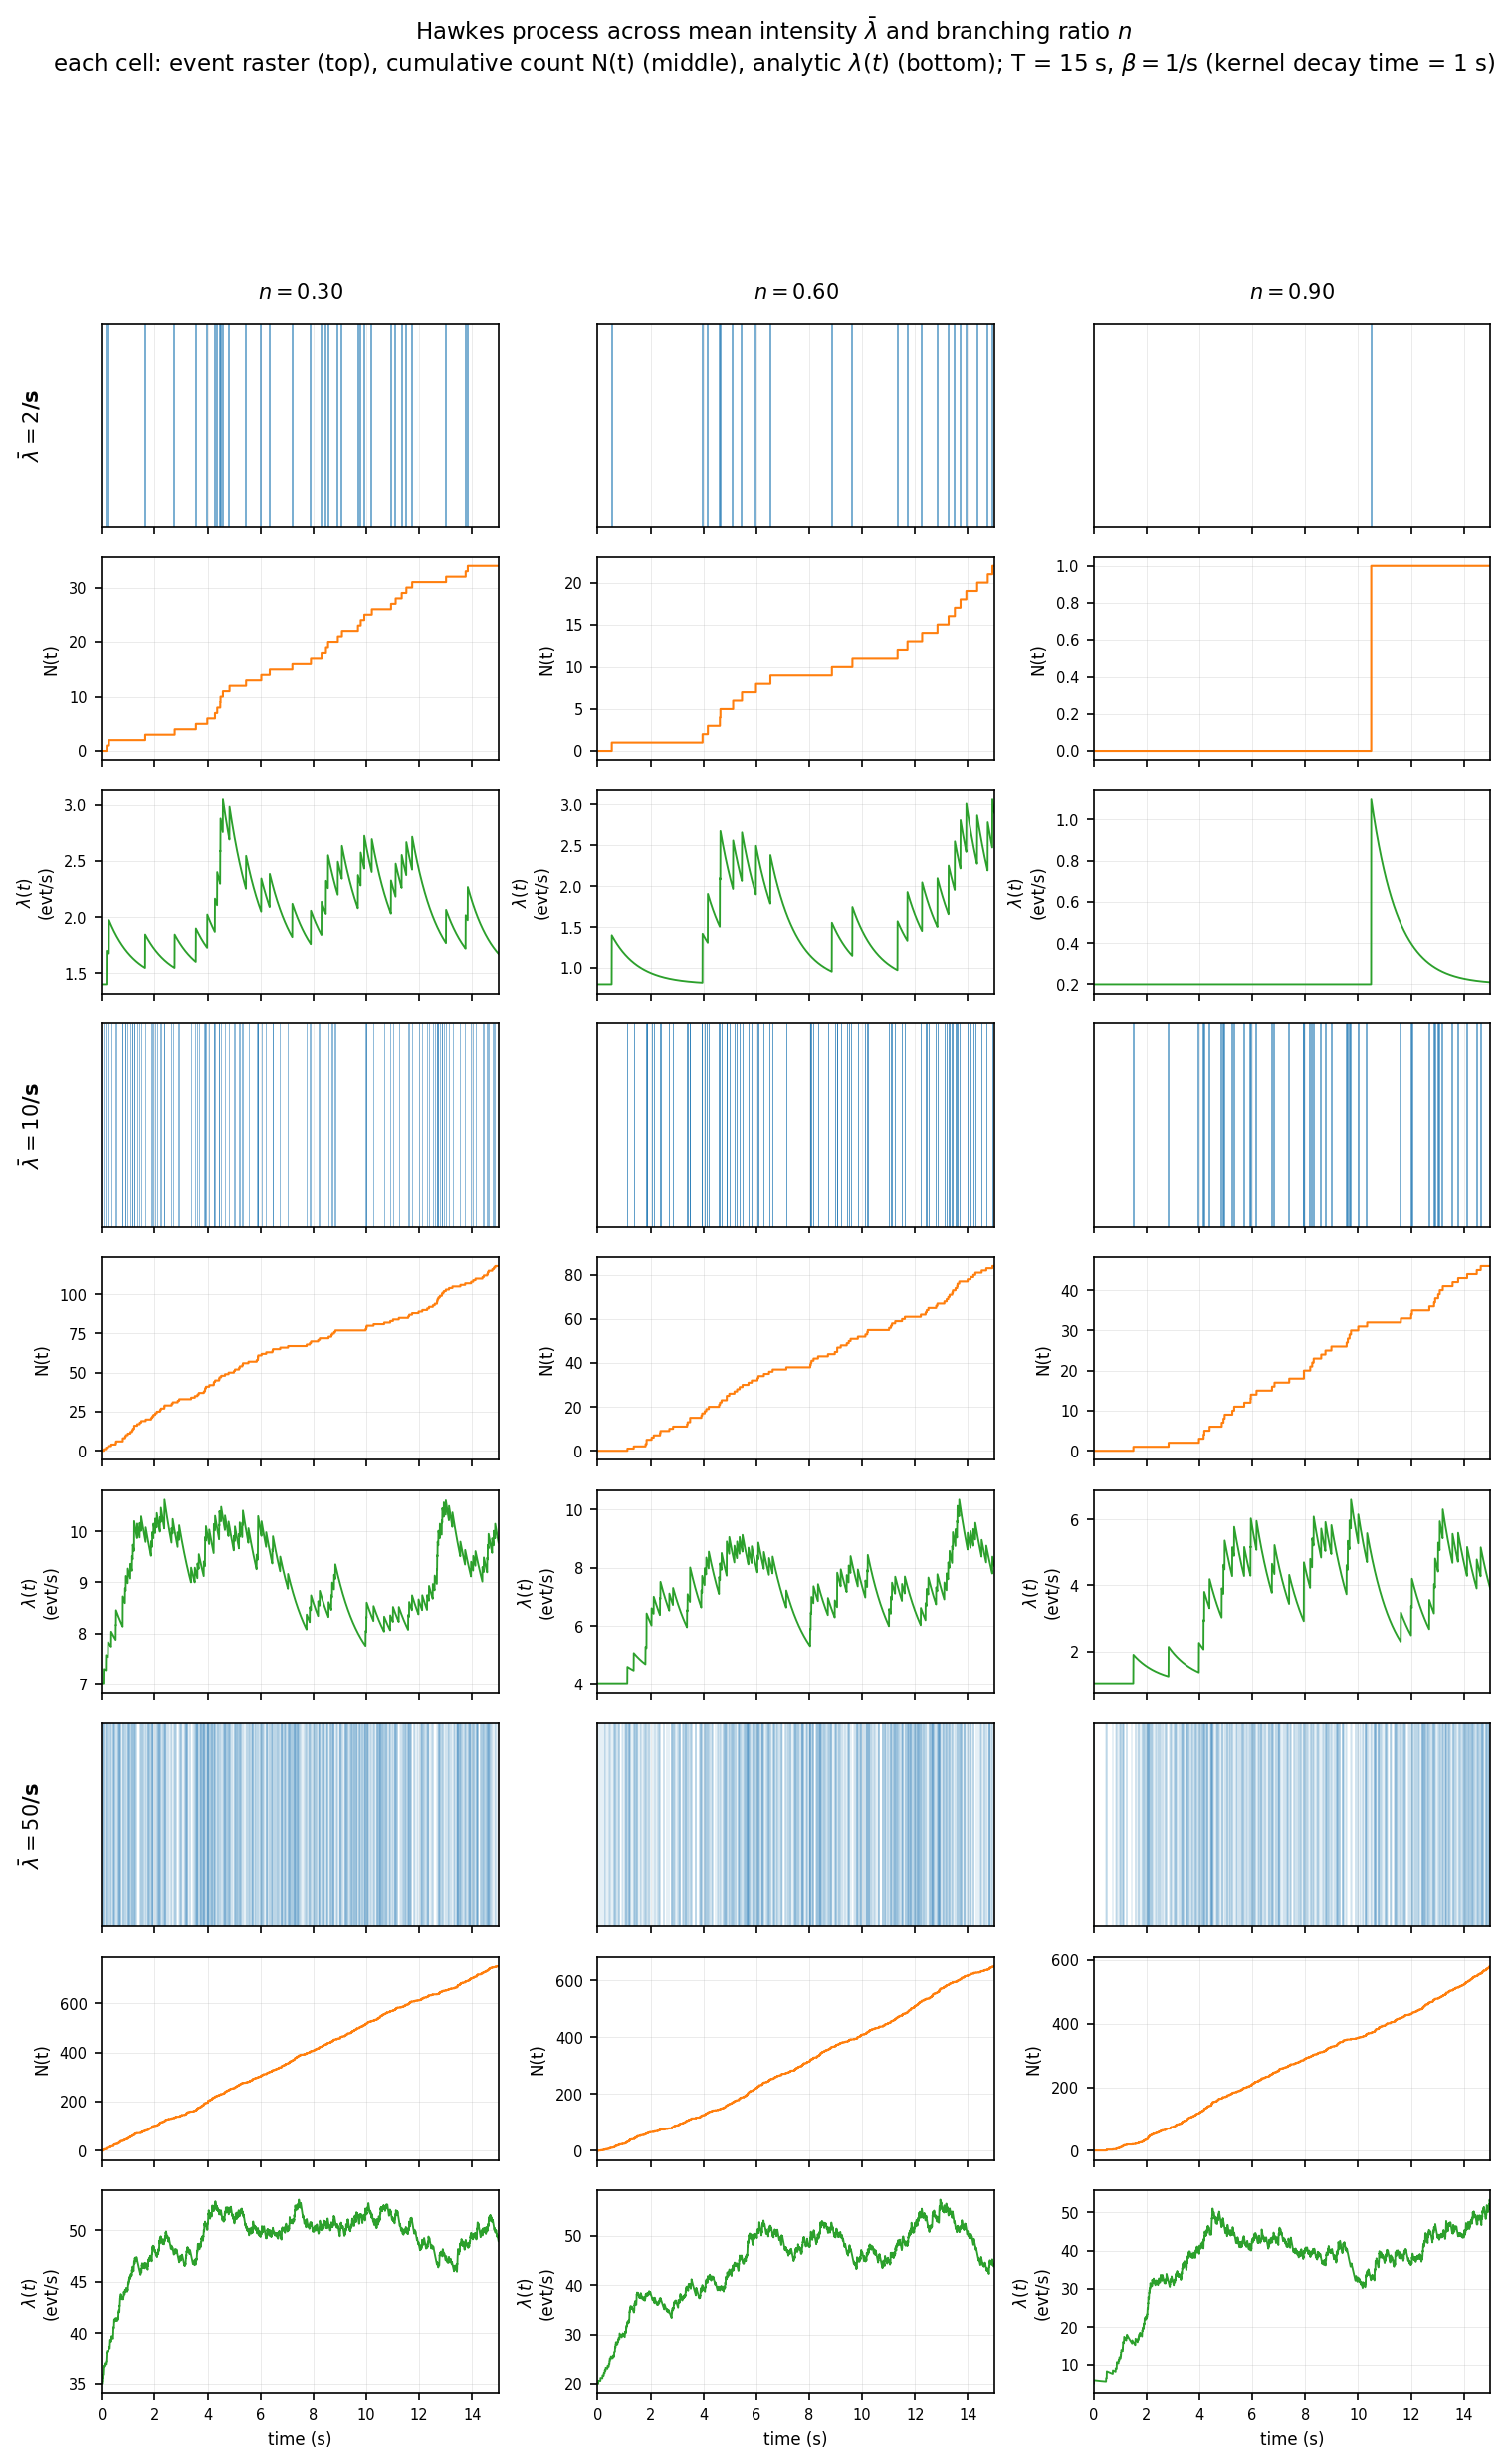
\includegraphics[width=\textwidth,height=0.72\textheight,keepaspectratio]{figs/hawkes_grid_3x3.png}
    \caption{Simulated exponential-kernel Hawkes processes. Each cell stacks the event
    raster (top), the cumulative count $N(t)$ (middle) and the intensity $\lambda(t)$
    (bottom). Rows: mean rate $\bar\lambda \in \{2, 10, 50\}$ events per second. Columns:
    branching ratio $n \in \{0.30, 0.60, 0.90\}$. Ogata thinning over $15$\,s with
    $\beta = 1/\mathrm{s}$; generator \texttt{make\_hawkes\_grid.py}, seed fixed per
    cell. The time scale is chosen for legibility; the kernel fitted on the corpus decays
    about four orders of magnitude faster.}
    \label{fig:hawkes-grid}
\end{figure}

\subsection{Three signatures that separate Poisson, renewal and Hawkes processes}
\label{app:pp-why-hawkes}

\emph{(i) An excess of short gaps.} On the corpus $73\%$ of packet gaps are shorter than a
tenth of the mean gap; any exponential gives $9.52\%$. A Hawkes process produces such an
excess, but so does a renewal process with a heavy-tailed gap distribution, so this
signature rejects Poisson without identifying self-excitation. On this feed the gap
shuffle keeps the whole excess (Table~\ref{tab:hawkes-diag}), and
Section~\ref{sec:exchange} traces the tightest gaps to the publisher sending consecutive
transactions one period apart.

\emph{(ii) Correlated gaps.} Under self-excitation, short gaps tend to follow short gaps
and long gaps follow long ones, so the gap autocorrelation is positive. A renewal process
has independent gaps and zero autocorrelation at every lag. A rate that varies slowly
over the window also produces positive gap correlation; the one-second-binned null $B$ of
Section~\ref{sec:setup-nulls} separates that case.

\emph{(iii) Burstiness that grows with the time scale.} The Fano factor $F(\tau)$ rises
with $\tau$ on a Hawkes process and levels off on a Poisson or renewal process.
Clustering is then not a feature of one time scale but looks similar over decades of
$\tau$. A slowly varying rate can also make $F(\tau)$ rise, which is the effect
\citet{filimonovsornette2015} warn about.

\subsection{Fano factor}
\label{app:pp-fano}

For a bin width $\tau$, cut the observation interval into $K$ disjoint bins and let
$C_k = N(k\tau) - N((k-1)\tau)$ be the count in bin $k$. The Fano factor is
$$F(\tau) = \frac{\mathrm{Var}[C_k]}{\mathrm{E}[C_k]}.$$
For a Poisson process $F(\tau) = 1$ at every $\tau$. For a renewal process with
finite-variance gaps $F(\tau)$ tends to the squared coefficient of variation of the gaps
as $\tau$ grows, a constant. For a clustered process $F(\tau) > 1$ and, under
self-excitation or a varying rate, it keeps growing with $\tau$. The measure is named
after U.~Fano, who introduced it in 1947 for fluctuations in counts of ions. On the
corpus $F(\tau)$ grows from $52$ at $0.1$\,s to about a thousand at $60$\,s, and the
shuffled stream is flat at about $17$ (Table~\ref{tab:hawkes-diag}).

\begin{figure}[H]
    \centering
    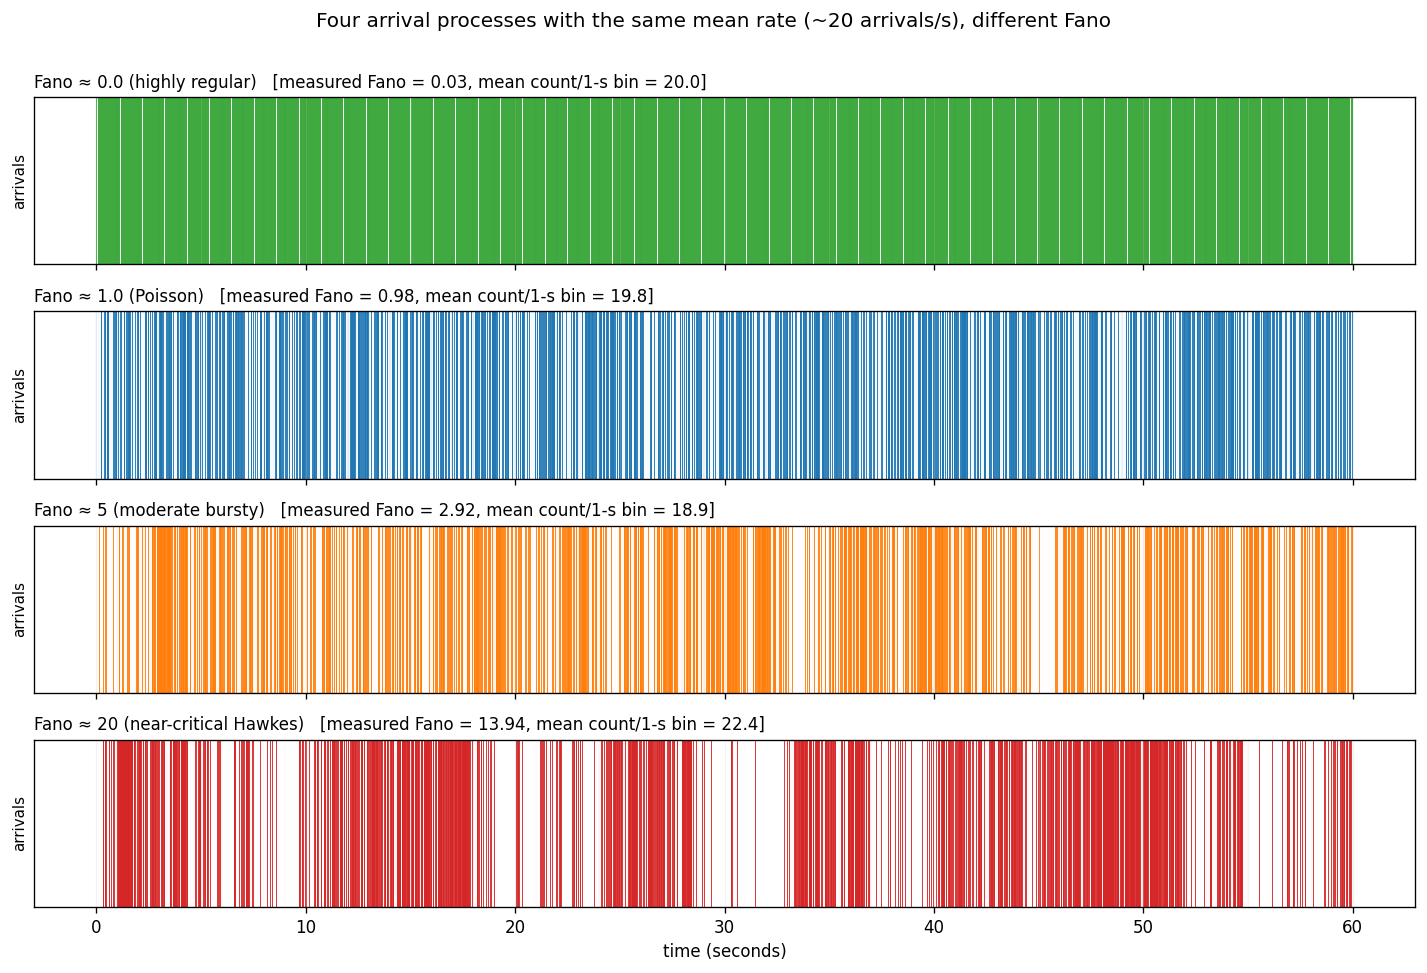
\includegraphics[width=\textwidth]{figs/rasters_by_fano.png}
    \caption{Four simulated processes at the same mean rate of about $20$ per second.
    Top row ($F \approx 0$, highly regular): near-lattice arrivals, nearly equal bin
    counts. Second row ($F \approx 1$, Poisson): the reference. Third row ($F \approx 3$,
    moderate Hawkes): visible clumping. Bottom row ($F \approx 14$, near-critical Hawkes):
    pronounced bursts and long quiet stretches, bin counts from near zero to over $50$.}
    \label{fig:rasters-fano}
\end{figure}

\begin{figure}[H]
    \centering
    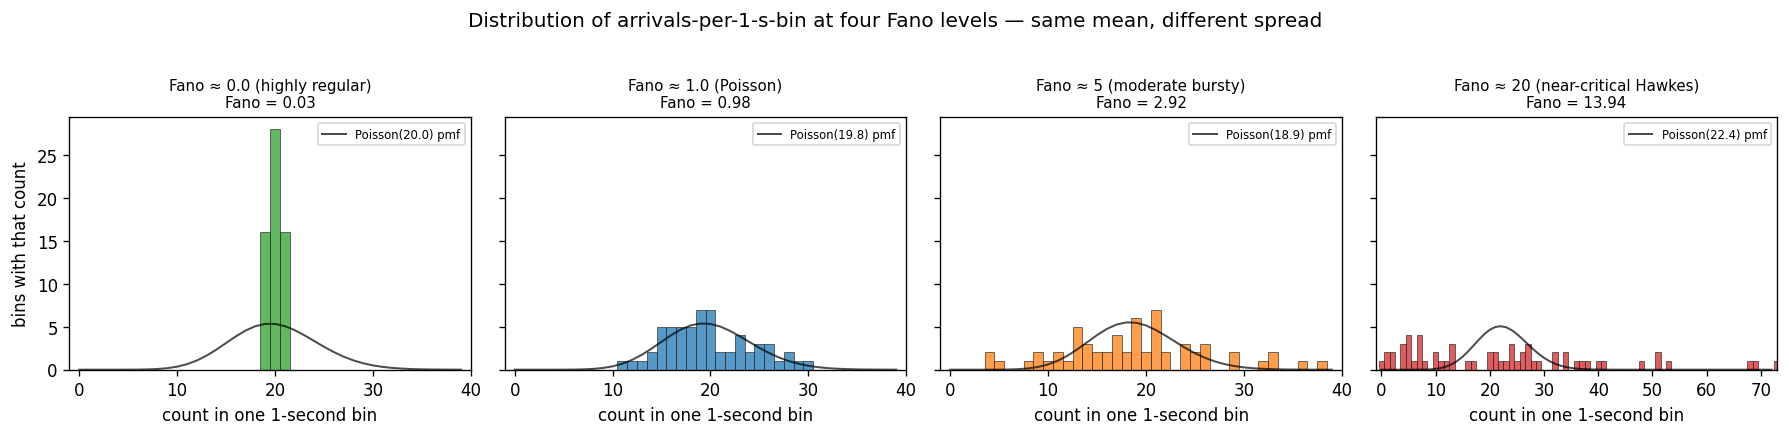
\includegraphics[width=\textwidth]{figs/count_hists_by_fano.png}
    \caption{Distribution of arrivals per one-second bin (bars) for the four processes of
    Figure~\ref{fig:rasters-fano}, with the Poisson distribution at the same mean
    overlaid (curve). $F \approx 0$: narrower than Poisson. $F \approx 1$: matches
    Poisson. $F > 1$: wider than Poisson, with extra mass in both tails. The NQ packet
    stream of the corpus has $F(1\,\mathrm{s}) = 108$ (Table~\ref{tab:hawkes-diag}),
    far wider than any panel shown.}
    \label{fig:counthist-fano}
\end{figure}

\subsection{Hurst exponent from the scaling of the Fano factor}
\label{app:pp-hurst}

When the Fano factor grows as a power of the bin width,
$$F(\tau) \sim \tau^{2H - 1},$$
the exponent $H$ is the Hurst exponent. $H = 0.5$ means no long-range dependence (Poisson,
and renewal with finite-variance gaps); $0.5 < H < 1$ means long-range dependence, with
clustering that looks similar across time scales; $H$ near $1$ means very long memory. It
is estimated by least squares on the log-log plot,
$$\log F(\tau) = (2H - 1)\log \tau + c + \varepsilon,$$
so $H = (\text{slope} + 1)/2$. On the corpus $H = 0.74$ (Table~\ref{tab:hawkes-diag}).

\begin{figure}[H]
    \centering
    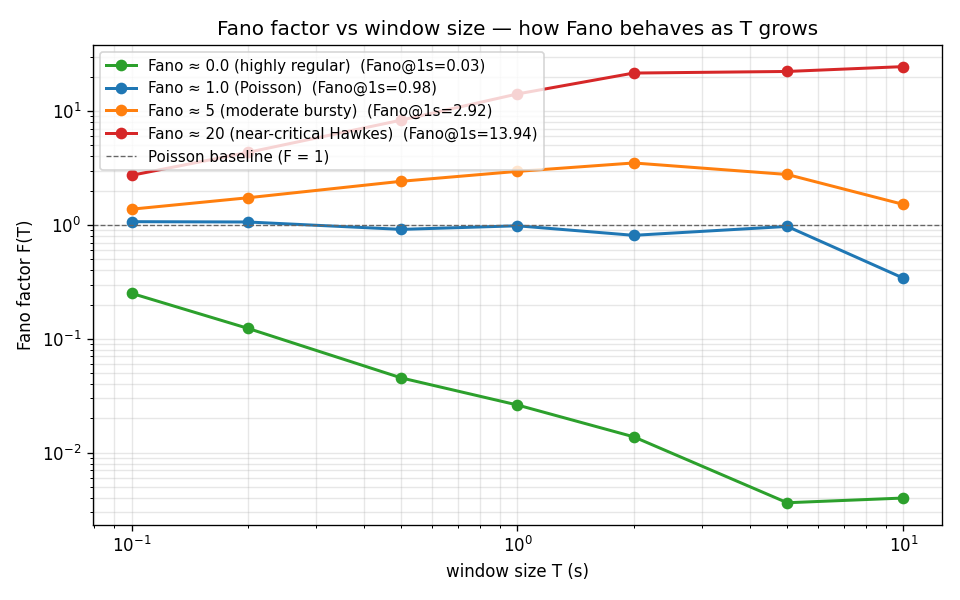
\includegraphics[width=0.75\textwidth]{figs/fano_scaling.png}
    \caption{$F(\tau)$ against $\tau$ on logarithmic axes for four simulated processes.
    Regular: $F$ near zero. Poisson: flat at $1$. Moderate Hawkes: rising. Near-critical
    Hawkes: steeper rise, with slope about $0.5$, i.e.\ $H \approx 0.75$.}
    \label{fig:fano-scaling}
\end{figure}

Shuffling the gap sequence preserves the gap distribution exactly and destroys the
ordering, and with it any long-range dependence: on the shuffled stream $H \to 0.5$. On
the corpus the shuffle takes $H$ from $0.74$ to $0.50$, so the long-range dependence
lives in the order of the gaps (Section~\ref{sec:setup-hawkes}).

\subsection{Fitting an exponential-kernel Hawkes process}
\label{app:mle}

The input is a sorted list of arrival times $t_1 < \cdots < t_m$ over a window
$[0, t_{\mathrm{end}}]$, and there are three parameters:
\begin{itemize}
    \item $\mu$, the \textbf{background rate}: arrivals per second with no recent history;
    \item $\alpha$, the \textbf{jump}: the rise in intensity, in arrivals per second, at
each arrival;
    \item $\beta$, the \textbf{decay rate}: each jump fades as $e^{-\beta u}$, with decay
time $1/\beta$.
\end{itemize}
Fitting means choosing the parameters under which the observed timestamps are most
probable, i.e.\ maximising the log-likelihood \citep{ozaki1979}
\begin{equation}
\log L(\mu, \alpha, \beta) = \sum_{i=1}^m \log \lambda(t_i) - \int_0^{t_{\mathrm{end}}} \lambda(s)\, ds.
\label{eq:hawkes-loglik}
\end{equation}
The first term rewards high intensity at the times arrivals actually occurred; the second
penalises a model that predicts more arrivals than occurred. If $\alpha$ is too small the
model cannot explain the bursts; if $\alpha$ approaches $\beta$ it predicts more clustering
than there is; a wrong $\mu$ mis-explains the quiet periods.

For the exponential kernel both terms have closed forms computable in one pass. With
$$R_i = e^{-\beta(t_i - t_{i-1})}(1 + R_{i-1}), \qquad R_1 \equiv 0,$$
the intensity at each arrival is $\lambda(t_i) = \mu + \alpha R_i$, and the compensator is
$$\int_0^{t_{\mathrm{end}}} \lambda(s)\, ds = \mu\, t_{\mathrm{end}} + \frac{\alpha}{\beta}
\sum_{i=1}^m\!\big(1 - e^{-\beta(t_{\mathrm{end}} - t_i)}\big).$$
Timestamps are shifted to the start of the window before fitting, so that the
exponentials do not underflow. The paper maximises the log-likelihood per window with
Nelder--Mead over $(\mu, \alpha, \beta)$ and checks the optimum with a reparameterised
L-BFGS-B fit (Section~\ref{sec:setup-hawkes}). From the fitted parameters follow the
branching ratio $n = \alpha/\beta$, the kernel decay time $1/\beta$, and the long-run
rate $\bar\lambda = \mu/(1 - n)$: the background rate amplified by $1/(1-n)$ through
self-excitation.

\subsection{Notation}
\label{app:pp-notation}

\begin{center}
\begin{tabular}{@{}ll@{}}
\toprule
symbol & meaning \\
\midrule
$\Omega$, $\mathcal{F}$, $\Pr$ & sample space, $\sigma$-algebra, probability \\
$\mathcal{F}_t$, $\mathcal{F}_{t^-}$ & everything observable up to $t$ inclusive, strictly before $t$ \\
$t_1, t_2, \ldots$ & arrival times \\
$N(t)$ & counting process, $\#\{i : t_i \leq t\}$ \\
$\lambda(t \mid \mathcal{F}_{t^-})$ & conditional intensity, arrivals per unit time \\
$\mu$ & background rate of a Hawkes process \\
$\phi(u)$ & Hawkes kernel \\
$\alpha$, $\beta$ & exponential-kernel jump and decay rate; decay time $1/\beta$ \\
$n = \int \phi$ & branching ratio; $n = \alpha/\beta$ for the exponential kernel \\
$\bar\lambda = \mu/(1-n)$ & long-run mean rate \\
$\Delta_i = t_i - t_{i-1}$ & interarrival gap \\
$\tau$ & bin width for counts (the service time is $T$) \\
$C_k$ & arrivals in bin $k$ \\
$F(\tau)$ & Fano factor, $\mathrm{Var}[C_k] / \mathrm{E}[C_k]$ \\
$H$ & Hurst exponent, $F(\tau) \sim \tau^{2H-1}$ \\
\bottomrule
\end{tabular}
\end{center}
